\documentclass[11pt]{article}

% Page geometry
\usepackage[margin=0.4in]{geometry}

% Typography
\usepackage[T1]{fontenc}
\usepackage{microtype}
\usepackage{multicol}
% Math
\usepackage{amsmath,amssymb,amsthm}

% Figures and tables
\usepackage{graphicx}
\usepackage{booktabs}
% Figures and tables
\usepackage{subcaption}
\usepackage{float}

% Make section headings smaller
\usepackage{titlesec}
\titleformat{\section}{\normalsize\bfseries}{\thesection}{1em}{}
\titleformat{\subsection}{\small\bfseries}{\thesubsection}{1em}{}
\titleformat{\subsubsection}{\footnotesize\bfseries}{\thesubsubsection}{1em}{}

% Make title smaller
\makeatletter
\renewcommand{\maketitle}{%
    \begin{center}
        {\normalsize \@title}\par
        \vskip 0.5em
        {\small \@author}\par
        \vskip 0.5em
        {\small \@date}\par
    \end{center}
}
\makeatother

% Make figure and table captions smaller
% \usepackage[font=small,labelfont=bf]{caption}
% Algorithms
\usepackage{algorithm}
\usepackage{algorithmic}

% References and links
\usepackage[colorlinks=true,linkcolor=blue,citecolor=blue,urlcolor=blue]{hyperref}
\usepackage[numbers]{natbib}

% Theorem environments
\newtheorem{theorem}{Theorem}
\newtheorem{lemma}[theorem]{Lemma}
\newtheorem{proposition}[theorem]{Proposition}
\newtheorem{definition}{Definition}

% Useful shortcuts
\newcommand{\R}{\mathbb{R}}
\newcommand{\E}{\mathbb{E}}
\newcommand{\argmin}{\operatorname{argmin}}
\newcommand{\argmax}{\operatorname{argmax}}

\renewcommand{\abstractname}{Summary}

\usepackage{xcolor}

% Make blockquotes italic and gray with a line at the end
\let\oldquote\quote
\let\endoldquote\endquote
\renewenvironment{quote}{\oldquote\itshape\color{gray}}{\par\noindent\rule{\linewidth}{0.4pt}\endoldquote}


\title{CS 148a Bonus Assignment}
\author{Arjun Sharma\\
\texttt{asharma3@caltech.edu}}
\date{}

\begin{document}

\maketitle

In my projects, I found that my ResNet CNN from project 2 performed the best, achieving 95.00\% validation accuracy with optimal hyperparameters. My DINO-downstream achieved 74.2\%, ViT achieved 72.9\% accuracy, and CLIP-downstream achieved 64.5\%. Validation accuracy was calculated over 15\% of the provided data that was held out during training.

We define validation error as $1 - \text{validation accuracy}$. We show the base-10 log of this error in the following plots.

\section{Log error and sample count}

Models were trained for 50 epochs with batch size 64.
\begin{figure}[H]
    \centering
    
\includegraphics[width=0.75\textwidth]{plots/plot1_samples.pdf}
    \caption{Overall, we see the expected log-linear relationship. The CNN, being trained from scratch, shows better scaling than the downstream models, which have smaller expressive power and rely more on the pre-trained feature extractors, which are not re-trained with respect to the training samples. The ViT was extremely sensitive to hyperparameters and the training setup here could not find a good parameter combination. }
\end{figure}

\section{Log error and parameter count}

It was most viable to change parameter count for the DINO downstream and CLIP models, since changing the CNN and ViT models from projects 2 and 3 would have required large scale architectural changes and taken too long to train.

My architecture for the downstream classifier for both of these was a 3-layer MLP with the form  
Linear(512, 256) $\to$ BatchNorm1d(256) $\to$ ReLU $\to$ Dropout $\to$ Linear(256, 128) $\to$ BatchNorm1d(128) $\to$ ReLU $\to$ Dropout $\to$ Linear(128, 10). I varied the dimension of the two hidden layers to vary the total parameter count for these experiments.

\begin{figure}[H]
    \centering
    
\includegraphics[width=0.75\textwidth]{plots/plot2_params.pdf}
    \caption{We see a log-linear scaling relationship between parameter count and error, as expected. DINO scales better since its features are, at least empirically, better adapted to the adversarial local structure in this dataset.}
\end{figure}

\section{Log error and inference time}

I measured the mean inference time for ten forward passes through the saved best checkpoints from each model and plotted them against log-val error of those checkpoints.

\begin{figure}[H]
    \centering
    
\includegraphics[width=0.75\textwidth]{plots/plot3_wallclock.pdf}
    \caption{The CNN is in the best quadrant: low inference time, low error. The ViT shows a similar error rate as the downstream classifiers but is much more expensive due to its quadratic compute scaling.}
\end{figure}

\section{Bonus plots}

I include plots ommitted from my report on project 2. In this project, I achieved 95.00\% validation accuracy locally and 81.37\% accuracy on the held-out Gradescope set. I found that a key part of this success was using \textit{synthetic data}, where I projected MNIST digits onto random backgrounds from the MNIST-in-the-wild training data to produce 6000 synthetic examples, which resulted in non-negligible (1-4\%) marginal improvements.

I was interested in analyzing why this worked. I needed to validate at least two claims: that the synthetic data did not interefere with the training process such that performance on the synthetic data tracked performance on the original data during training, and that the learned features over the training data were not meaningfully different across synthetic and real examples.

\begin{figure}[H]
    \centering
    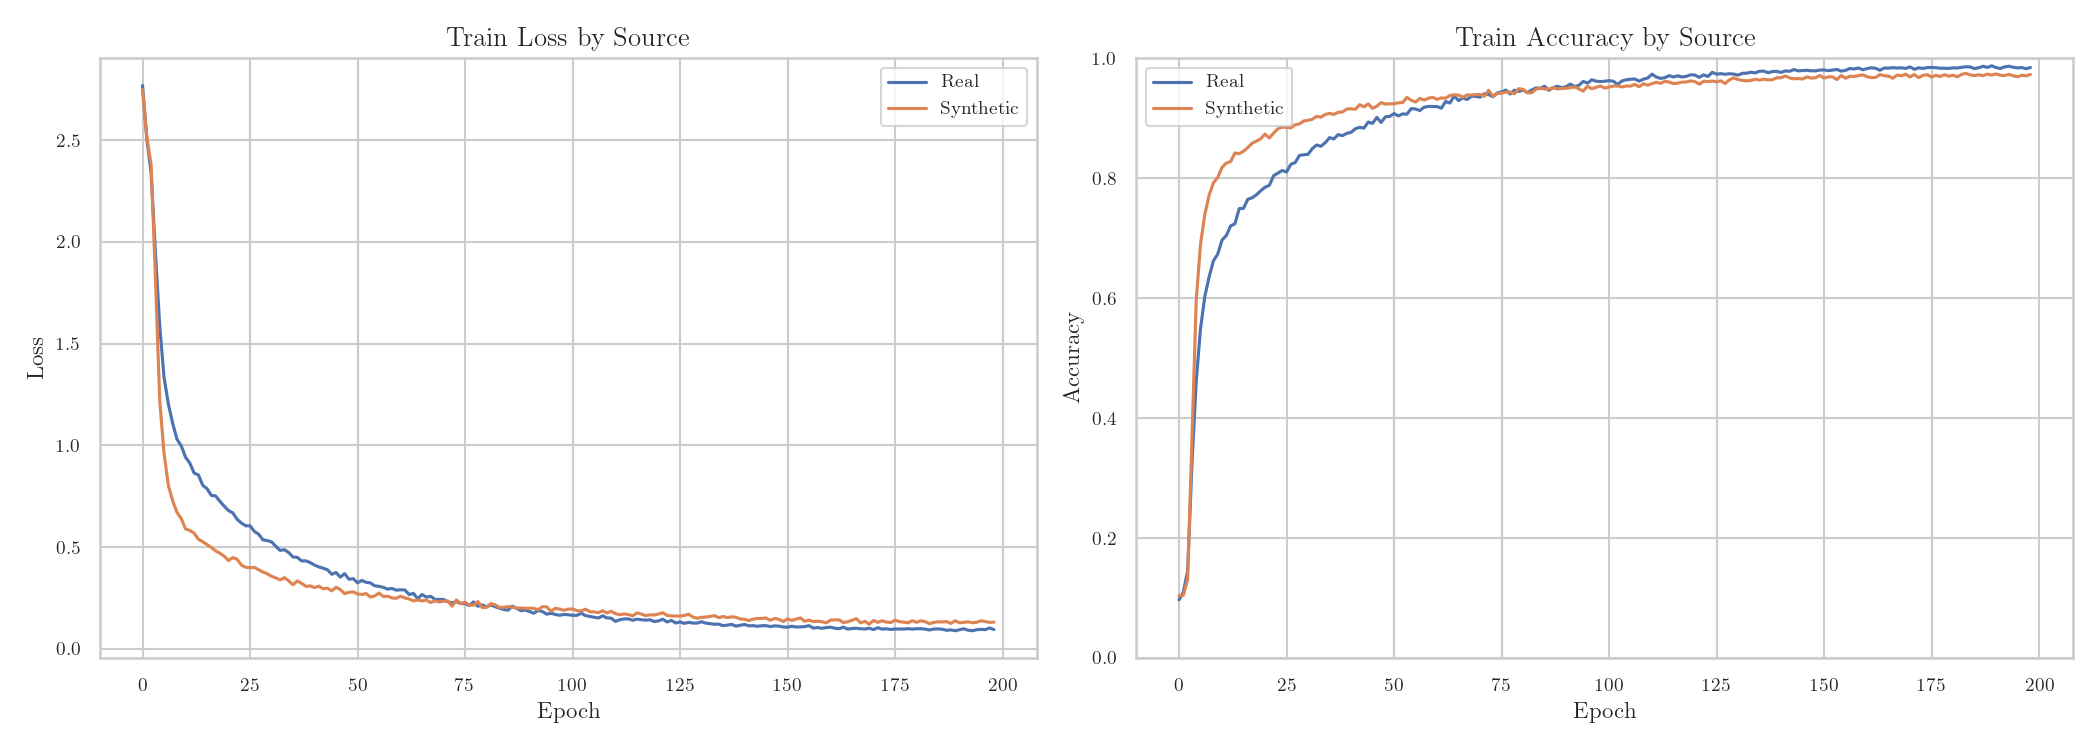
\includegraphics[width=0.75\textwidth]{plots/bonus/per_source.png}
    \caption{Training curves for the ResNet CNN over epochs broken up by source. We see that synthetic data is initially an easier target than the real data but eventually converges to the same performance, suggesting that it likely helps the model learn useful features initially with a more tractable digit structure.}
\end{figure}

\begin{figure}[H]
    \centering
    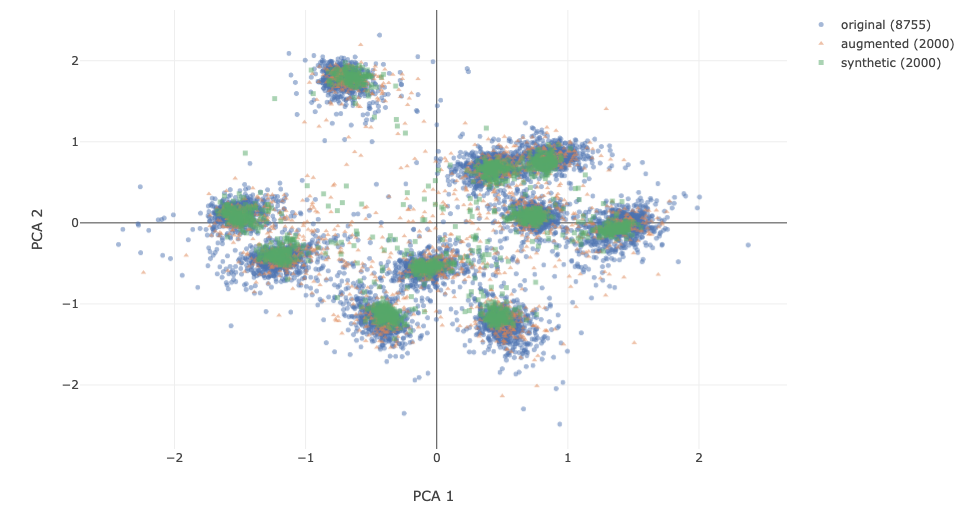
\includegraphics[width=0.8\textwidth]{plots/bonus/all-sources-overlay.png}
    \caption{A projection of the extracted features before the classification layer of the trained ResNet over the training data to the first two principal components. Overall, as expected, there are ten clusters corresponding to ten digit types. We want to ensure that the augmented data and synthetic data are not too far from the original data and broadly stay close to their original clusters. We see this is the case, and that the synthetic data plays a similar role as the augmented data, therefore allowing us to expand the size of the dataset and reduce overfitting risk even after gains from augmentation have saturated.}
\end{figure}

This visualization method is insightful in general in understanding the performance of my models. Applying it to the validation dataset, we can visualize the principled understanding of CNNs as feature extractors, whose representations in the final layer before classification are used to extract predictions. 

\begin{figure}[H]
 \centering
 \begin{subfigure}[t]{0.45\textwidth}
    \centering
    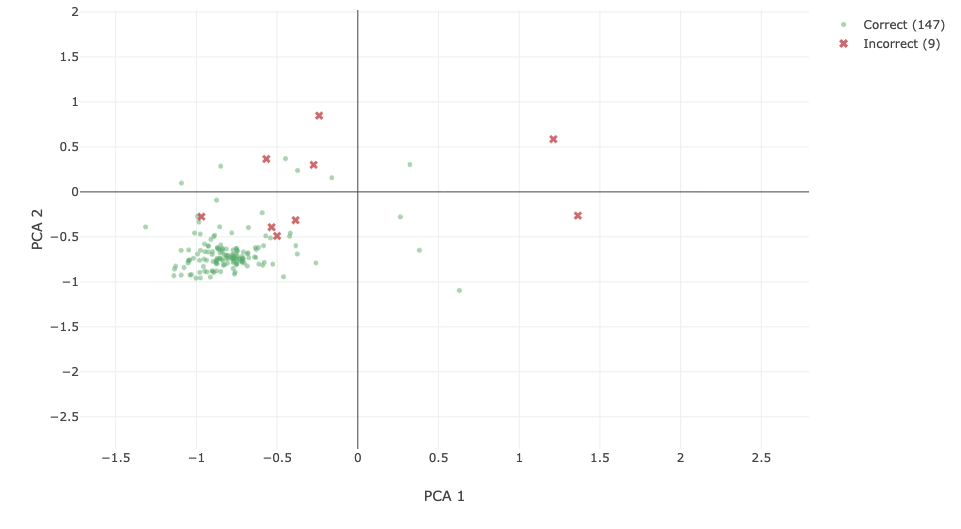
\includegraphics[width=\textwidth]{plots/bonus/class-3-preds.png}
    \caption{Class 3}
 \end{subfigure}
  \begin{subfigure}[t]{0.45\textwidth}
    \centering
    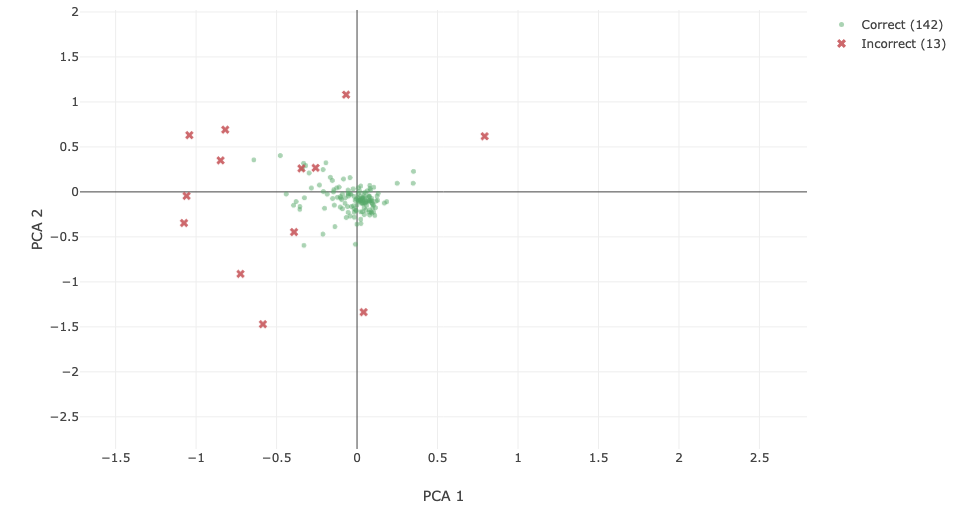
\includegraphics[width=\textwidth]{plots/bonus/class-8-preds.png}
    \caption{Class 8}
 \end{subfigure}
 \caption{Principal components of features extracted for validation examples for two classes. Notice that the correct examples are tightly clustered together (and, by inspection, are close to their clusters in the previous figure), and the incorrect examples have features far from the correct cluster. We see that they essentially violate they learned decision boundary over these extracted feature representations.}
\end{figure}

\appendix
\section{AI Usage}

I wrote all the analysis and designed all the experiments for this project, but used AI to orchestrate a lot of the experiments since they were largely reorganizations of my existing codebases. I include all prompts provided to Claude Code below.

First, I provided it a guidance file:
\begin{verbatim}
    You are in a subdirectory `bonus_project` of a directory `cs-148` containing work for a deep learning class. Ignore the `hw` folders.

Projects 2, 3, and 4 contain the setup for training deep neural network classifiers on an extremely adversarial dataset, which has been copied to data/dataset here.

The goal of this final subproject is to run 3 experiments to produce 3 plots:
1. Plot 1: Log Error vs. Log Sample countHow did the number of total training samples change the validation and training error?
2. Plot 2: Log Error vs. Log Parameter countHow does the error scale with the number of parameters?
3. Plot 3: Log Error vs. Wall ClockHow did the error scale with inference time? Use the same compute resource for all checkpoints,

My plan is to extract the CNN and ViT setups and re-run training experiments with different # sample counts and diferent depths. 

I will come up with a plan for plot 3 later. 

\end{verbatim}

\begin{enumerate}
    \item Open guidance/instructions.md. Read it. Survey the parent directory's subdirectories and start putting together a plan 
  for re-running experiments for the CNN from project 2 and ViT from project 3.  
  \item Execute this
  \item Run all the experiments necessary to generate and save all the plots I need for this project. Use seaborn with latex  
  font with color palette "deep". Make sure to save with dpi = 600.      
  \item Re-evaluate your estimate of how long things will take given the current rate of progress.            
  \item Kill the ViT test. Let's run these scaling tests for the models in project4 with the downstream DINO and downstream    
  CLIP. Enter plan mode if ncessary      
  \item Set up plot 3 - log error vs wall clock. We can do a really simple version of this. Just run K times - set K=10 -      
  forward passes through the best CNN chcekpoint from the project 2 directory, the best ViT checkpoint from the project    
  3, the best DINO and CLIP checkpoints from project 4.      
  \item Change it to re-generate these with inference time on a regular scale, not a log scale. Keep error on a log sclae.    
\end{enumerate}

\end{document}